\chapter{Introducción}
\pagenumbering{arabic} %Para empezar la numeración con números naturales

En este trabajo se hará un análisis estadístico de los datos recabados de las páginas de horarios de la Facultad de Ciencias de la UNAM, de los cuales se obtendrá un número estimado de alumnos, para cada materia de las carreras, del Departamento de Matemáticas, con el cual se podrán hacer aleatoriamente esqueletos de horarios que se calificarán de acuerdo a dicha demanda se resolverá el problema de asignación de horarios por medio del algoritmo genético. Con esto se desea disminuir el tiempo que se toma actualmente el hacer tanto los esqueletos de horarios como las asignaciones de grupos en la Facultad.

\section{Motivación}

Lo que motivó la realización de este trabajo es la aportación que se puede hacer a la Facultad, la cual nos parece de gran utilidad y para el beneficio de los futuros alumnos y la (posible) disminución del tiempo que toma realizar los esqueletos y la asignación de profesores en la Facultad.

Actualmente para hacer la asignación de horarios primero se reune el comité encargado de dicha tarea para realizar manualmente los esqueletos de los horarios, éstos se dan a conocer a los profesores y ellos eligen diferentes opciones de materias y posibles horas en las cuales les gustaría impartir sus clases. Una vez que los profesores han elegido, se vuelve a hacer una o varias juntas para la asignación final de los horarios que se hace de manera manual.

Se tienen dos tipos de profesores, los de base y los de asignatura. Los profesores de base, por contrato, deben de cubrir ciertas horas de clase por lo que al momento de hacer la asignación, éstos tienen prioridad sobre los profesores de asignatura. Finalmente se publican los horarios a los alumnos.

Una vez que los alumnos han elegido las materias que les gustaría tomar deben de ir con el profesor y él o ella les debe de firmar su tira de materias en caso de que el cupo del salón lo permita, en caso de que el alumno no consiga la firma de la materia que desea deberá buscar una segunda o tercera opción o incluso tener que meterla en algún semestre posterior.

La principal razón por la cual los profesores no firman las tiras de materias es porque el número de alumnos que desean inscribirse a su clase es mayor al número de lugares disponibles en el salón asignado. Es por ello que el trabajo que hemos realizado depende de la demanda de alumnos por materia y por horario.



\section{Definición de conceptos}

Las siguientes son las definiciones que se utilizarán a lo largo del trabajo:

\textbf{Materia:} Curso impartido en la Facultad de Ciencias por algún profesor.

\textbf{Horario:} Hora en la que se imparte alguna materia.

\textbf{Esqueleto:} Conjunto Materia-Horario.

\textbf{Asignación:} Conjunto Materia-Horario-Profesor.

\textbf{Grupo:} Clave con la que se identifica una asignación.

\textbf{Turno Matutino:} Comprende las clases impartidas de 7:00-14:00hrs incluyendo la clase de 14:00-15:00hrs.

\textbf{Turno Vespertino:} Comprende las clases impartidas de 15:00-21:00hrs incluyendo la clase de 21:00-22:00hrs.


\section{Nomenclatura}

$m:$ Número de materias que se van a impartir

$p:$ Número de profesores que van impartir alguna materia

$c:$ Número de salones de clase que se pueden ocupar

$i:$ Índice para profesores, $i \in \{ 1, 2, 3, \ldots, p \}$

$j:$ Índice para materias, $j \in \{ 1, 2, 3, \ldots, m \}$

$k:$ Índice para salones, $k \in \{ 1, 2, 3, \ldots, c \}$

$h:$ Índice para las horas del día, $h \in \{ 1, 2, 3 \ldots, 15\}$

$U_{j,i,h,k}:$ Utilidad de que el profesor $i$ imparta la materia $j$ en el salón $k$ a la hora $h$

$x_{j,i,h,k}:$ Variable binaria que vale $1$ si la materia $j$ es impartida por el profesor $i$ en el salón $k$ a la hora $h$ y cero en otro caso

$V_{j,i}:$ Variable binaria que vale $1$ si la materia $j$ puede ser impartida por  el profesor $i$ y cero en otro caso

$V_{j,k}:$ Variable binaria que vale $1$ si la materia $j$ puede impartirse en el salón $k$ y cero en otro caso

$s:$ Semestre a simular

$k:$ Número de semestres que se tienen como ventana de información

\textit{m\_grande:} Matriz en la que se guarda la información por semestres

$r:$ Matriz \textit{m\_filtrada}, submatriz de \textit{m\_grande}

\textit{vec\_sem\_sig:} Vector con los semestres que se van a simular

$X_{4}:$ Analizar presentación: Hacer varias pruebas con distintas combinaciones y elegir el mejor estilo/presentación

$X_{14}:$ Revisar/Investigar al respecto del problema y resolverlo

$num\_sim:$ Número de simulaciones de la demanda de alumnos para $s$

$:$ 

$:$ 

$:$ 

$:$ 

$:$ 

\section{Planteamiento del problema}

En el problema de asignación de horarios se quiere asociar un profesor con una materia, un salón y un horario. Existen trabajos que han aborado este problema desde otro punto de vista, por ejemplo Yazdani, Naeri y Zeinali, en su artículo \textit{Algorithms for university course scheduling problems} (\ref{Yazdani}), proponen un modelo en el cual se toman 2 decisiones: la asignación de profesor por materia y el salón en el cual se va a impartir cada materia.

Con la función objetivo planteada en dicho modelo se desea maximizar la utilidad de que el profesor $i$ imparta la materia $j$, más la utilidad de que el profesor $i$ dé clases el día $t$, más la utilidad de la materia $j$ por ser impartida en el día $t$.

Dos diferencias principales entre su modelo y el que proponemos en este trabajo son:

\begin{enumerate}
\item[1)] No tomamos en cuenta el día en el que se imparte la materia porque suponemos que todas las materias se imparten de lunes a viernes, a la misma hora, en el mismo salón.

\item[2)] Deseamos maximizar la utilidad de que el profesor $i$ imparta la materia $j$ en el salón $k$ a la hora $h$.
\end{enumerate}

%El problema que se tiene es un problema maximización en el cual se consideran:

Los elementos que consideramos en nuestro modelo son:

\begin{itemize}
\item[-] Esqueletos de horario: Matriz de 15 renglones con las horas (7-8, 8-9, $\ldots$, 21-22) y tantas columnas como materias. En la entrada $(i,j)$ contiene el número de grupos simulados de la i-ésima hora para la materia $j$.

\item[-] Función calificadora de esqueletos: Califica de acuerdo a qué tan bien o que tan mal se cubre la demanda de los alumnos esperados.

\item[-] Conjunto de materias: Nombres de las materias impartidas en la FC.

\item[-] Conjunto de profesores: Nombres de profesores de base y de asignatura.
\end{itemize}

\begin{enumerate}[i)]
\item Variables de decisión:

$ x_{j,i,h,k} =
  \begin{cases}
1  & \quad \text{si la materia } j \text{ es impartida por el profesor  } i,\\
   &\quad \text{ en el salón } k, \text{ a la hora } h\\
0  & \quad \text{e.o.c. } \\
\end{cases}
$

\item Función objetivo: (se desea maximizar la utilidad)

\begin{equation*}
\text{máx} \,\, z =  \,\, \displaystyle \sum_{i=1}^{p} \sum_{j=1}^{m} \sum_{k=1}^{c} \sum_{h=1}^{15} x_{j,i,h,k} U_{j,i,h,k} \,\,\,\, \text{s. a}
\end{equation*}

\item Restricciones:
  
\begin{eqnarray}
\displaystyle \sum_{i=1}^{p} \sum_{k=1}^{c} \sum_{h=1}^{15} x_{j,i,h,k} &=& 1  \,\,\,\,\,\,\, \forall \,\, j\\
\displaystyle \sum_{j=1}^{m} \sum_{k=1}^{c} x_{j,i,h,k} &\leqslant& 1 \,\,\,\,\,\,\, \forall \,\, i,h\\
\displaystyle \sum_{i=1}^{p} \sum_{j=1}^{m} x_{j,i,h,k} &\leqslant& 1 \,\,\,\,\,\,\, \forall \,\, k,h\\
\displaystyle \sum_{k=1}^{c} \sum_{h=1}^{15} x_{j,i,h,k} &\leqslant& V_{i,j} \,\,\,\,\,\,\, \forall \,\, i,j\\
\displaystyle \sum_{i=1}^{p} \sum_{h=1}^{15} x_{j,i,h,k} &\leqslant& V_{j,k}  \,\,\,\,\,\,\, \forall \,\, j,k\\
x_{j,i,h,k}, \,\, V_{j,i}, \,\, V_{j,k} &\in& \{0,1\} \,\,\,\,\,\,\, \forall \,\, j,i,h,k
\end{eqnarray}
\end{enumerate}

Con las restricciones del tipo $(1)$ aseguramos que todas las materias sean dadas. Con las del tipo $(2)$ se asegura que cada profesor no tenga más de un curso por hora. Las restricciones del tipo $(3)$ nos indican que se puede impartir máximo una materia en cada salón por hora. Con las del tipo $(4)$ aseguramos que los profesores tengan asignadas materias que puedan impartir. Las restricciones del tipo $(5)$ especifican que cada materia es asignada a un salón donde pueda impartirse esa clase. Finalmente con las restricciones del tipo $(6)$ se especifica que las variables utilizadas son binarias.

En el planteamiento se tienen dos tipos de restricciones: duras y suaves, las restricciones duras son las que nos permiten tener soluciones factibles al cumplirlas en su totalidad y las restricciones suaves nos permiten evaluar la calidad de las diferentes soluciones, usualmente están asociadas a preferencias y se cumplen en la medida de lo posible, pero no afectan la factibilidad de las soluciones.

El conjunto de soluciones se presenta por medio de la matriz \textit{mat\_asignaciones} la cual es una matriz de cuatro columnas y tantos renglones como materias se tengan. En el i-ésimo renglón se tiene la información de la i-ésima materia con su respectivo profesor, horario y salón asignados. En la tabla \ref{EjAsig} se muestra un ejemplo del resultado de la asignación.

\begin{table}[h]
\centering
\begin{tabular}{|c|c|c|c|}
 \hline 
 Materia & Profesor & Horario & Salón \\ 
 \hline 
 Inferencia Estadística & Margarita Chávez Cano & 9-10 & O123 \\ 
 \hline 
 Estadística II & Jaime Vázquez Alamilla & 10-11 & 001 (Yelizcalli) \\ 
 \hline 
 Estadística Bayesiana  & Ruth Fuentes García & 11-12 & P110 \\ 
 \hline 
 Estadística III  & Lizbeth Naranjo Albarrán & 13-14 & Aula Magna P \\ 
 \hline 
 \end{tabular}  
\caption{\textit{Ejemplo de asignación}}\label{EjAsig}
\end{table}


\section{Objetivos}

El primer objetivo del trabajo es hacer dos funciones, una que genere esqueletos de horarios y otra que que genere una asignación de profesores por materia y horario que cubra la demanda de alumnos estimada para un semestre dado.

Los esqueletos de horarios son utilizados para simular una posible elección de materias y horarios de los profesores para finalmente hacer la asignación correspondiente a la hora, materia, profesor y salón de cada grupo.

El segundo objetivo es disminuir el tiempo utilizado actualmente para la realización de la asignación de horarios.


\section{Datos a analizar}

Para poder realizar un análisis adecuado de los datos, se hicieron dos divisiones de ellos. La primera fue con respecto al tipo de semestre, par o impar y la segunda se hizo con respecto al turno, matutino o vespertino.

Se tomó la información de la materia de \textit{Probabilidad I}, desde el semestre 2015-1 hasta el 2020-1, para explicar la elección de las divisiones. Cabe aclarar que dicha materia en la carrera de Actuaría es una materia obligatoria de tercer semestre.

Veamos primero la división de acuerdo a semestres pares e impares.

En la figura \ref{ParImparProbaI} se tiene una gráfica en la que la línea azul representa el número de alumnos de los semestres impares y la línea roja representa el número de alumnos de los semestres pares. Se observa que en todo momento el número de alumnos de los semestres impares es mayor al número de alumnos de los semestres pares. Lo cual nos interesa porque al momento de simular se debe de tomar en cuenta que siempre el número de alumnos totales de semestres impares debe de ser mayor al número total de alumnos de los semestres pares.

\begin{figure}[h]
\centering
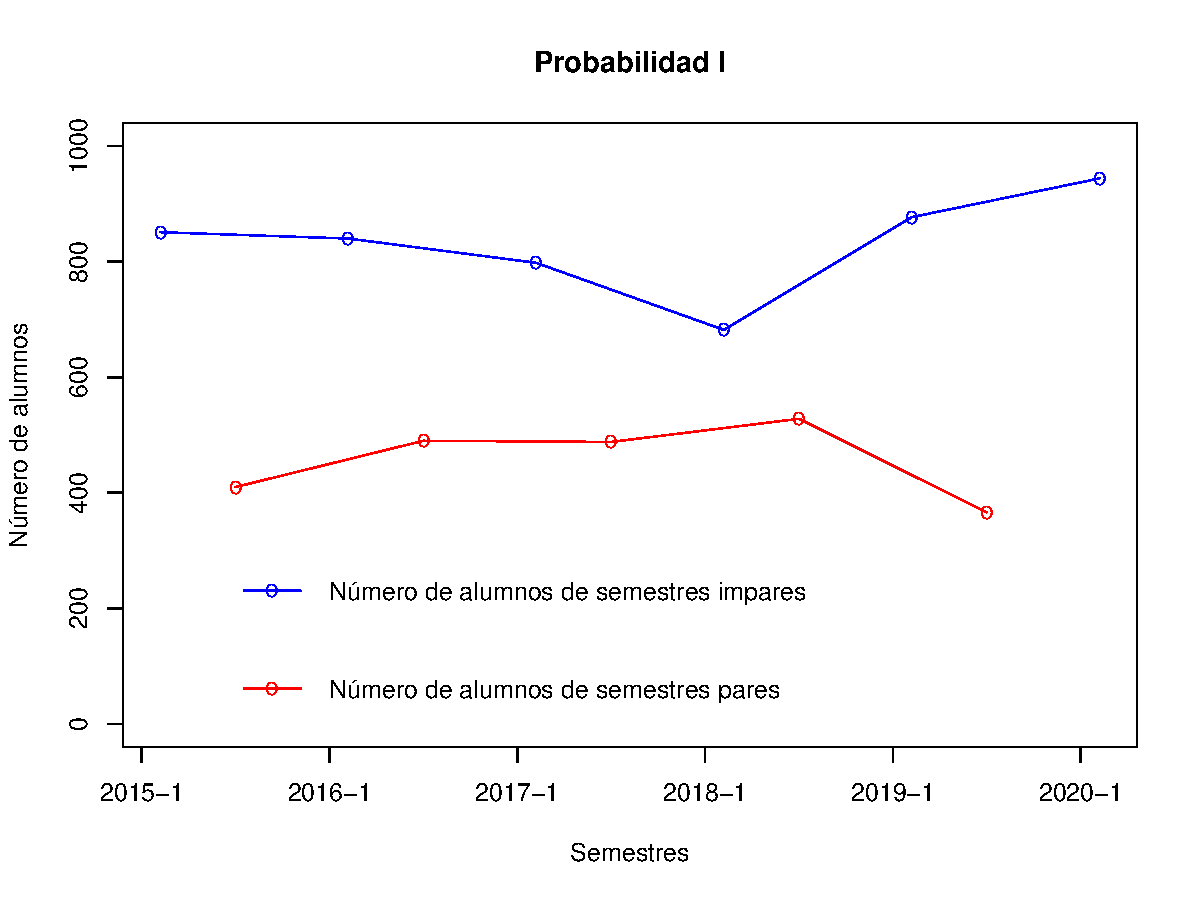
\includegraphics[scale = 0.8]{num_alum_sem_par_impar_Proba_I.pdf} %width=\textwidth
\caption{\textit{Número de alumnos totales por semestres pares e impares}} \label{ParImparProbaI}
\end{figure}

Continuando con los datos de \textit{Probabilidad I} se obtuvo la gráfica de la figura \ref{HistAlumParImparProbaI} que contiene dos histogramas, las barras rojas representan el número de alumnos por grupo de semestres pares y las barras azules representan el número de alumnos por grupo de semestres impares.

Las líneas que se encuentran sobre los histogramas son densidades estimadas que se ajustan a los histogramas. Algunos datos que se pueden obtener de esas densidades son por ejemplo que alrededor del $20\%$ de los grupos de los semestres pares tienen aproximadamente de $60$ a $70$ alumnos y que alrededor del $3\%$ de los grupos de los semestres impares tienen entre 150 y 180 alumnos.

\begin{figure}[h]
\centering
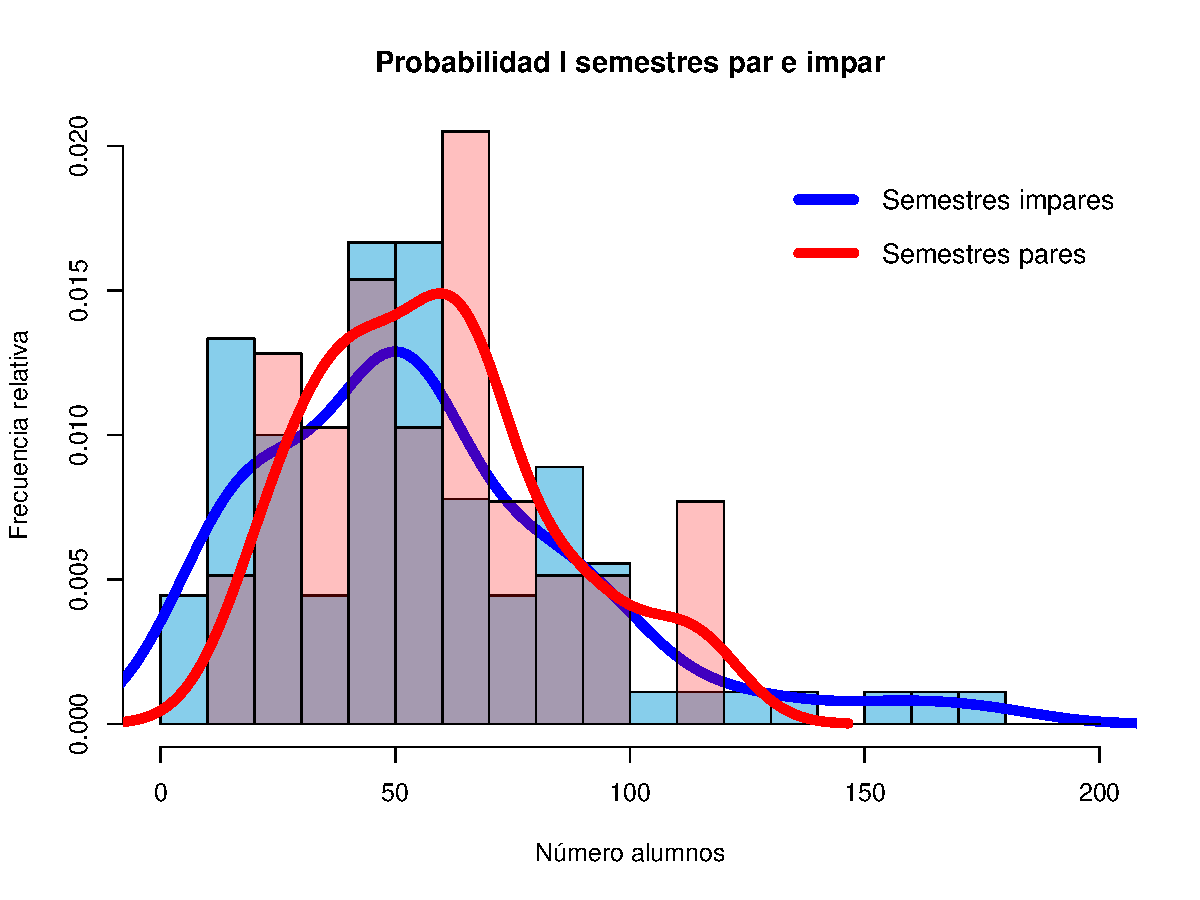
\includegraphics[scale = 0.8]{histograma_FR_num_alum_sem_par_impar_Proba_I.pdf} %width=\textwidth
\caption{\textit{Histograma del número de alumnos por semestre}} \label{HistAlumParImparProbaI}
\end{figure}


Ahora veamos la segunda división de acuerdo a los turnos matutino y vespertino.

En la gráfica de la figura \ref{num_alum_x_turno_Proba_I} la línea azul representa el número de alumnos del turno matutino y la línea roja representa el número de alumnos del turno vespertino. Se puede observar que en todo momento el número de alumnos del turno matutino es mayor al número de alumnos del turno vespertino, esto impacta en el hecho de que por semestres la varianza en el turno matutino es mucho mayor que en el turno vespertino lo cual indica que en el turno vespertino se tiene prácticamente el mismo número de alumnos sin importar si la materia pertenece a un semestre par o impar, a diferencia de lo que ocurre en el turno matutino en donde si influye el hecho de que la materia corresponda a un semestre par o impar.


\begin{figure}[h]
\centering
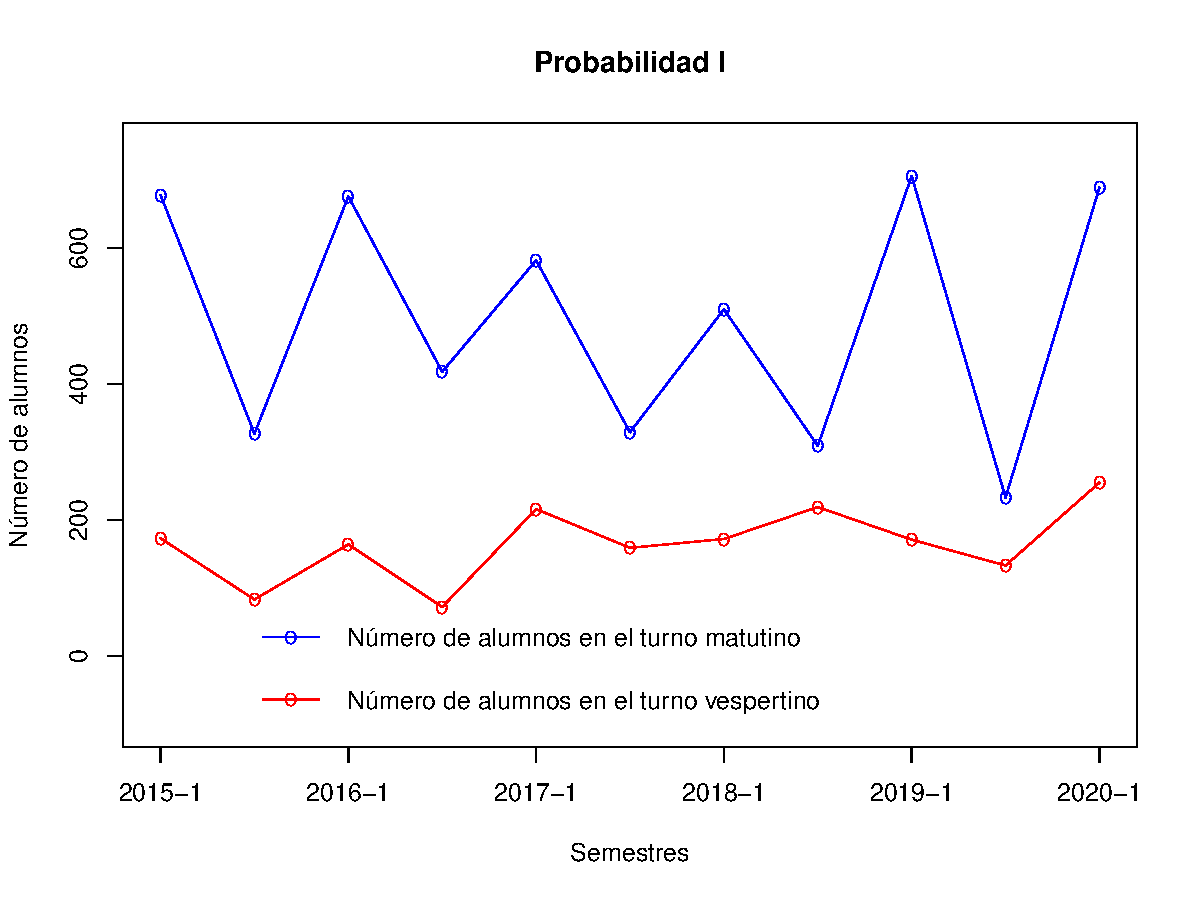
\includegraphics[scale = 0.7]{num_alum_x_turno_Proba_I.pdf} %width=\textwidth
\caption{\textit{Número de alumnos por turno}}\label{num_alum_x_turno_Proba_I}
\end{figure}

Al igual que en la primera división se obtuvo una gráfica que contiene dos histogramas, sobre los cuales se tienen 2 líneas con  densidades estimadas que se ajustan a los histogramas. Dicha gráfica se observa en la figura \ref{HistAlumTurnoProbaI} en la cual podemos ver que las barras rojas representan el número de alumnos del turno vespertino y las barras azules representan el número de alumnos del turno matutino.

Notamos que en este caso las densidades son completamente diferentes. Algunos datos que se pueden obtener de dichas densidades son por ejemplo que alrededor del $20\%$ de los grupos del turno vespertino tienen aproximadamente entre 10 y 20 alumnos y un poco más del $10\%$ de los grupos del turno matutino tienen entre 80 y 90 alumnos.

\begin{figure}[h]
\centering
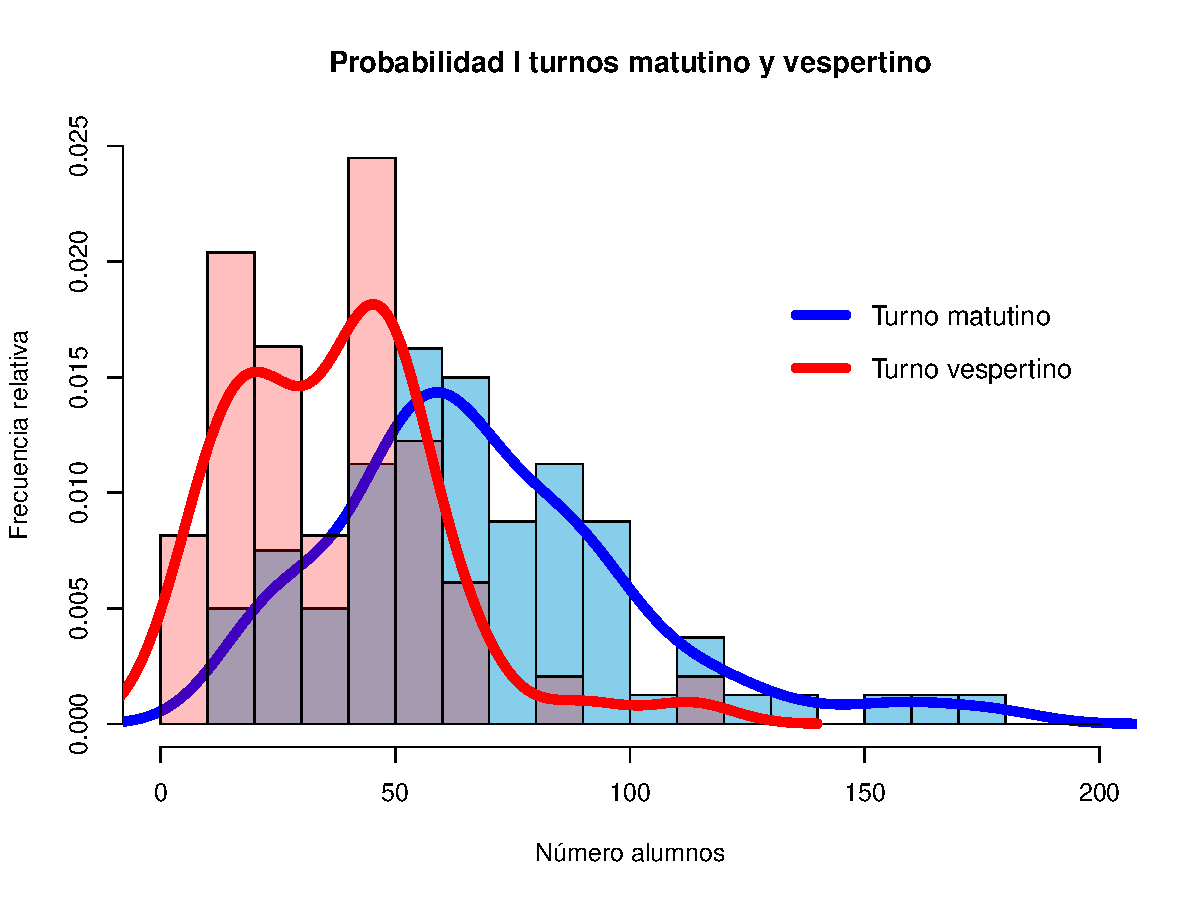
\includegraphics[scale = 0.7]{histograma_FR_num_alum_x_turno_Proba_I.pdf} %width=\textwidth
\caption{\textit{Histograma del número de alumnos por turno}}\label{HistAlumTurnoProbaI}
\end{figure}

Con los resultados observados se obtuvieron los grupos de datos $G_{1}, G_{2}, G_{3}, G_{4}$, para hacer los análisis estadísticos, los cuales se definen en la tabla \ref{GposDatos}.

\begin{table}[h]
\centering
\begin{tabular}{|c|c|c|}
\hline 
Sem. $\setminus$ Turno & Matutino & Vespertino \\ 
\hline 
Impar & $G_{1}$ & $G_{2}$ \\ 
\hline 
Par & $G_{3}$ & $G_{4}$ \\ 
\hline 
\end{tabular} 
\caption{\textit{Grupos de datos}}\label{GposDatos}
\end{table}
